%!TEX root = main-beamer.tex
%###############################################################################
\begin{document}
%###############################################################################

\maketitle           % makes title for article only
\frame{\titlepage}   % makes title for presentation only


% Structuring a talk is a difficult task and the following structure
% may not be suitable. Here are some rules that apply for this
% solution: 

% - Exactly two or three sections (other than the summary).
% - At *most* three subsections per section.
% - Talk about 30s to 2min per frame. So there should be between about
%   15 and 30 frames, all told.

% - A conference audience is likely to know very little of what you
%   are going to talk about. So *simplify*!
% - In a 20min talk, getting the main ideas across is hard
%   enough. Leave out details, even if it means being less precise than
%   you think necessary.
% - If you omit details that are vital to the proof/implementation,
%   just say so once. Everybody will be happy with that.


\section*{Introduction}
%----------------------
  We demonstrate data transmission of 10 Gbit/s on-off keying modulated
  1550 nm signal through a long-range dielectric-loaded surface
  plasmon polariton waveguide (LR-DLSSPw) structure with negligible signal
  degradation. In the experiment the bit error rate penalties do not exceed
  0.6 dB over the 15 nm wavelength range and received optical power
  between –7 and 3 dBm.
  \begin{frame}<presentation>{Abstract}
    \begin{itemize}
      \item[\cmark] We demonstrate 10\,Gbit/s transmission over\\
            300\,$\mu$m-long nanooptic waveguide
            \vspace{3mm}
      \item[\cmark] The signal degradation is almost negligible\cite{kharitonov_data_2014}
    \end{itemize}
  \end{frame}


% ######################################################################



\section{Motivation}
%-------------------
  In this section we briefly describe waveguides that we were using; we
  mention what are their possible application.
  \begin{frame}{Motivation – unique waveguiding structure}
    LR-DLSPPW – long-range dielectric-loaded surface plasmon-polariton\\
    \hfill waveguide \cite{volkov_long-range_2011}
    \begin{columns}
      \column[c]{0.42\textwidth}
        \begin{figure}
          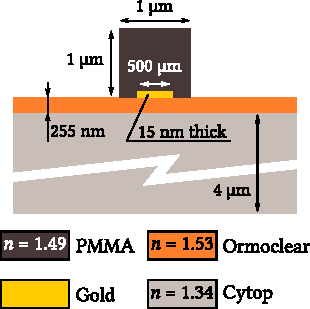
\includegraphics[width=43mm]{wg_profile.pdf}
        \end{figure}
      \column[c]{0.58\textwidth}
        \begin{block}{Configuration – sandwiched structure}
          \begin{itemize}
           \item Gold stripe for mode confinement
           \item PMMA ridge on gold stripe
           \item Small longitudinal $\vec{E}$-component
           \item $\sim 1.0\,\mu{}m$ mode field diameter
          \end{itemize}
        \end{block}
    \end{columns}
  \end{frame}
  
  On the next slide we present the problem~-- these waveguides have huge
  insertion losses. It is not clear if a modulated signal can be recovered
  after such waveguide.

  \begin{frame}{Motivation: properties of the LR-DLSPPW structure}
    \vspace{-3mm}
    \begin{columns}
      \column[t]{0.48\textwidth}
        \begin{block}{Key features:}
          \begin{itemize}
            \item Strong mode confinement% $\sim 1\,\mu{}m$
            \item mm-long propagation range
            \item Low losses at sharp bends
            \item Stim. emission of plasmonic modes for loss compensation
          \end{itemize}
        \end{block}
      \column[t]{0.40\textwidth}
        \begin{block}{Promising applications:\\
                      Compact telecom devices}
          \begin{itemize}
            \item Modulators / Resonators
            \item Couplers / Multiplexers
            \item Integrated plasmonics
            \item Optical interconnects
          \end{itemize}
        \end{block}
    \end{columns}
    \pause
    \begin{center}
      \begin{minipage}{0.8\textwidth}
        \begin{alertblock}{Experiment: transmission of modulated signal}
          Test LR-DLSSPW in the standard telecom environment:
          \begin{itemize}
            \item 1550\,nm
            \item 10\,Gbit/s, \textsc{on-off} keying
            \item several channels
          \end{itemize}
        \end{alertblock}
      \end{minipage}
    \end{center}
  \end{frame}


% ######################################################################




\section{Materials and Methods}
%------------------------------
  This section presents an overview of used materials and methods
  \begin{frame}{Methods – our goals}
    \begin{block}{Test LR-DLSPPW in a telecom system}
    \begin{columns}
      \column[t]{0.55\textwidth}
        \begin{itemize}
          \item Couple 1550\,nm light to waveguide
          \item Transmit 10\,Gbit/s modulated signal
        \end{itemize}
      \column[t]{0.45\textwidth}
        \begin{itemize}
          \item Evaluate channel cross-talk
          \item Find \emph{bit-error rate} (BER)\\
                \hfill penalties~~~
        \end{itemize}
    \end{columns}
    \vspace{-5mm}
        \begin{center}
          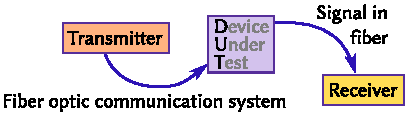
\includegraphics[width=0.6\textwidth]{simple_FOCS.pdf}
        \end{center}
    \end{block}
      \begin{exampleblock}{What is \emph{BER}?}
        \emph{BER} – probability of incorrect bit detection\\
      \end{exampleblock}

  \end{frame}

  
 
  \subsection{Concepts} % (fold)
  %--------------------
  \label{sub:concepts}
  \begin{frame}{Concept of BER penalty}
    \begin{block}{Difference between DUT and ideal attenuator in terms of BER}
      \begin{center}
        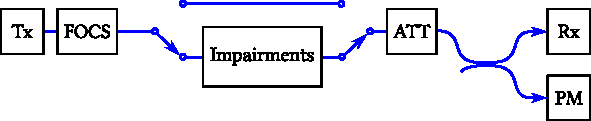
\includegraphics[width=0.7\textwidth]{BER_impairment.pdf}
      \end{center}
    \end{block}
    \begin{center}
      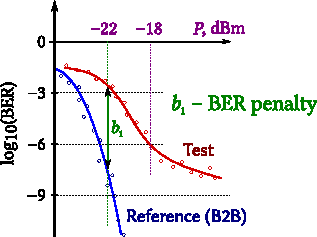
\includegraphics[width=0.75\linewidth]{BER_penalties.pdf}
    \end{center}
  \end{frame}
  % subsection concepts (end)



  \subsection{Experimental techniques} % (fold)
  \label{sub:experimental_techniques}
  
  \begin{frame}{Experimental techniques}
    \begin{block}{Prototype of fiber optic communication system}
      \begin{center}
        \only<1>{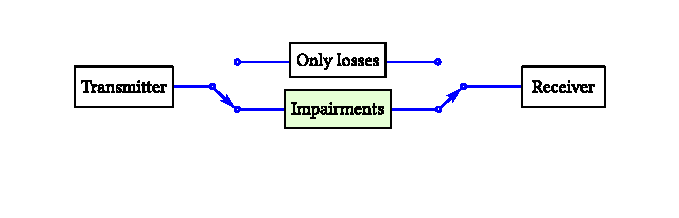
\includegraphics[width=\textwidth]{BERsetup1.pdf}}
        \only<2>{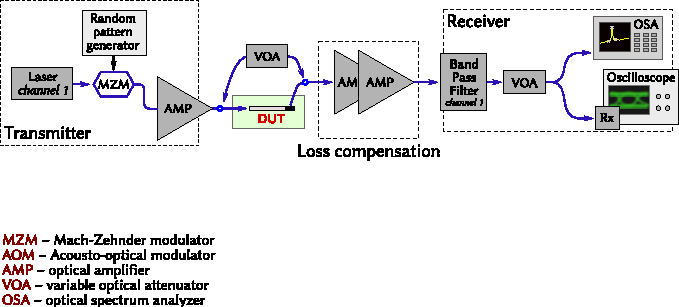
\includegraphics[width=\textwidth]{BERsetup2.pdf}}
        \only<3>{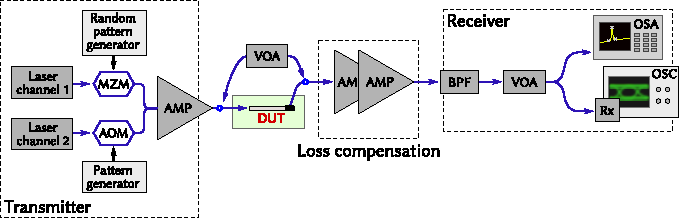
\includegraphics[width=\textwidth]{BERsetup3.pdf}}
        \only<4>{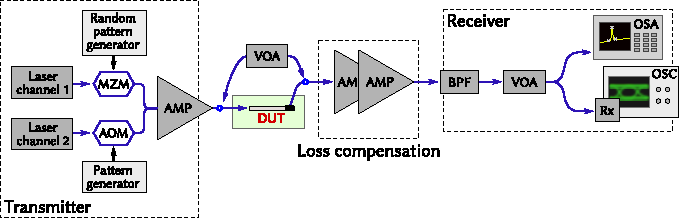
\includegraphics[width=\textwidth]{BERsetup3.pdf}\\
                 \vspace{-5mm}\hspace{35mm}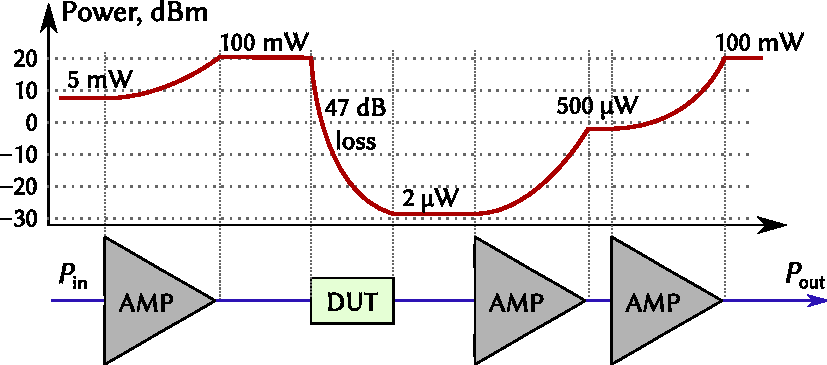
\includegraphics[width=0.6\textwidth]{Pbudget.pdf}}
      \end{center}
    \end{block}
  \transdissolve<2>
  \transwipe<3>
  \transwipe<4>
  \end{frame}


  \begin{frame}{Experimental techniques}
               {Light coupling to LR-DLSSPW}
    \begin{columns}
      \column[c]{0.4\textwidth}
        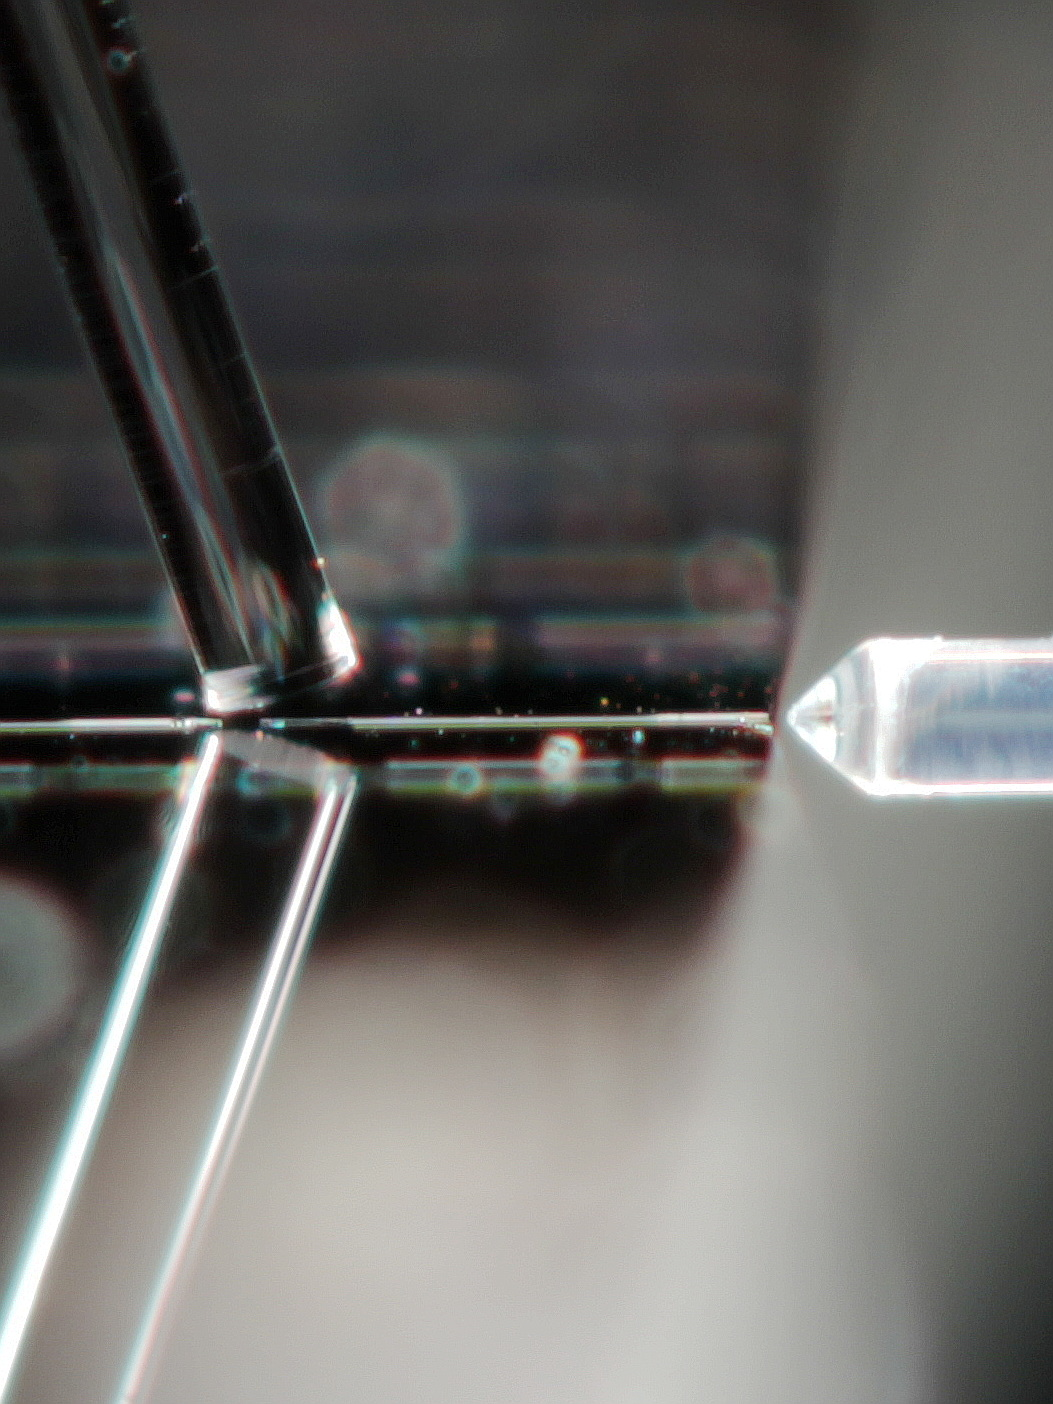
\includegraphics[width=\textwidth]{coupling_alignment_VIS.jpg}
      \column[c]{0.6\textwidth}
        \begin{center}
          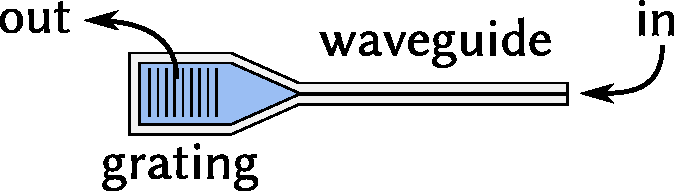
\includegraphics[width=0.7\textwidth]{wg_coupling.pdf}          
        \end{center}
        \vspace{-2mm}
        \begin{itemize}
          \item Input coupling with lensed fiber
          \item Collection with cleaved fiber
        \end{itemize}
        \vspace{4mm}
        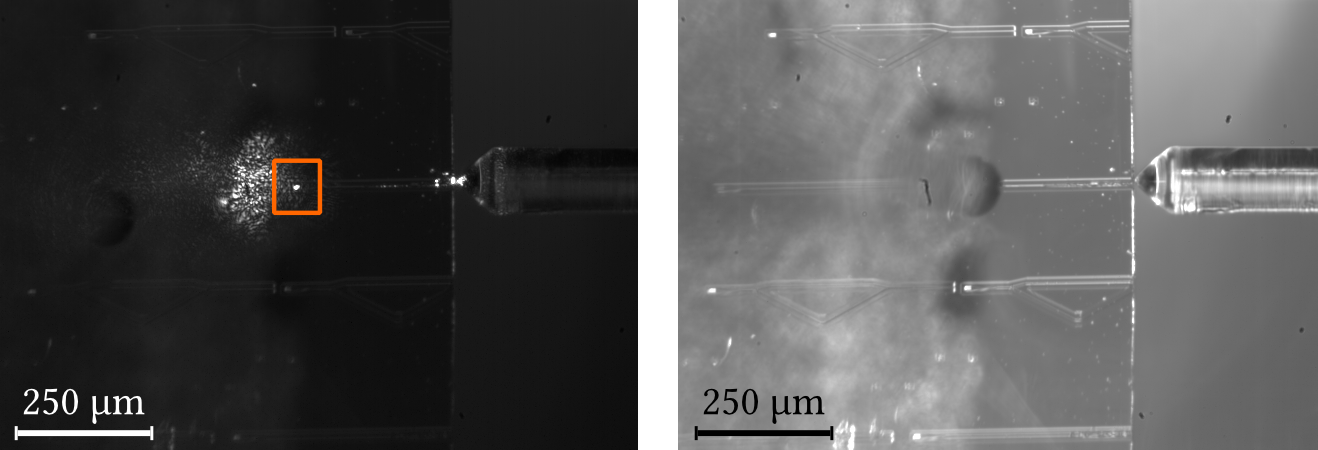
\includegraphics[width=\textwidth]{coupling_alignment_IR.png}
    \end{columns}
  \end{frame}

  \begin{frame}{Experimental techniques}
               {Light coupling to LR-DLSSPW}
    \begin{columns}
      \column{0.42\textwidth}
        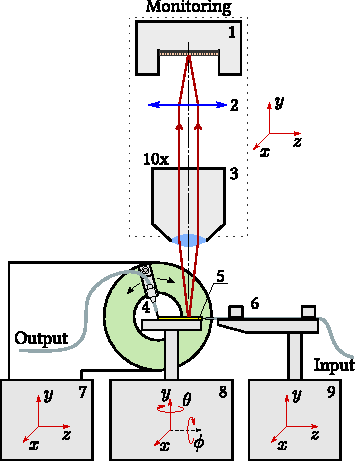
\includegraphics[height=7cm]{coupling_setup.pdf}
      \column{0.48\textwidth}
        \begin{block}{Light coupling system}
          \begin{itemize}
            \item Piezo-driven stages
            \item IR microscope with huge WD
            \item Photocamera with macrolens
          \end{itemize}
        \end{block}
        \vspace{0mm}
        \begin{center}
          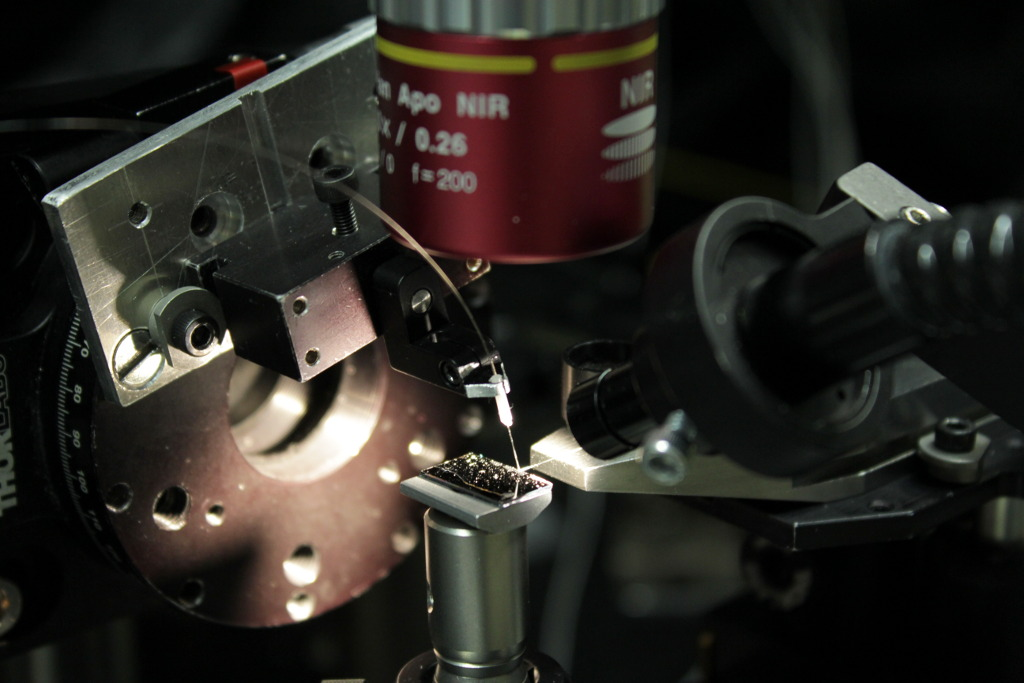
\includegraphics[width=\textwidth]{coupling.jpg}
        \end{center}
    \end{columns}
    \begin{center}
    \end{center}
  \end{frame}
  % subsection experimental_techniques (end)


  \subsection{Data processing} % (fold)
  \label{sub:data_processing}
  
  % subsection data_processing (end)
  \begin{frame}{Data processing techniques}
    \emph{Eye diagram} (left) is the overlay of all possible transitions
    \vspace{-1mm}
    \begin{center}
      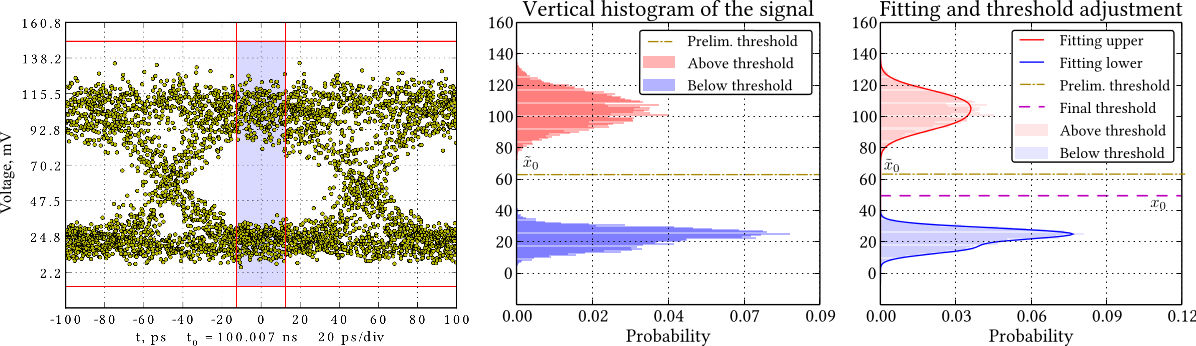
\includegraphics[width=\textwidth]{hist_processing_diagram_1200px.jpg}
    \end{center}
    \begin{columns}
      \column[c]{0.5\textwidth}
        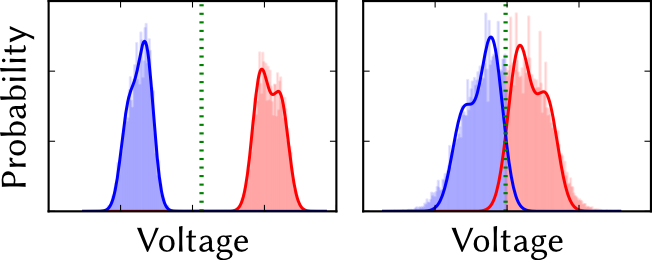
\includegraphics[height=22mm]{diff_fitting.png}\hspace{-4mm}
      \column[c]{0.45\textwidth}
        \vspace{-3mm}
        \begin{block}{BER is determined statistically}
          \begin{enumerate}
            \item Collect vertical histrogram
            \item Perform fitting
            \item Find area of overlap
          \end{enumerate}
        \end{block}
    \end{columns}
  \end{frame}



% ######################################################################





\section{Results and Contribution}
%---------------------------------
  \begin{frame}{Results and Contributinon}
               {Single and double channel transmission}
    \begin{block}{1549\,nm, channel spacing 0.4\,nm}
      \centering
      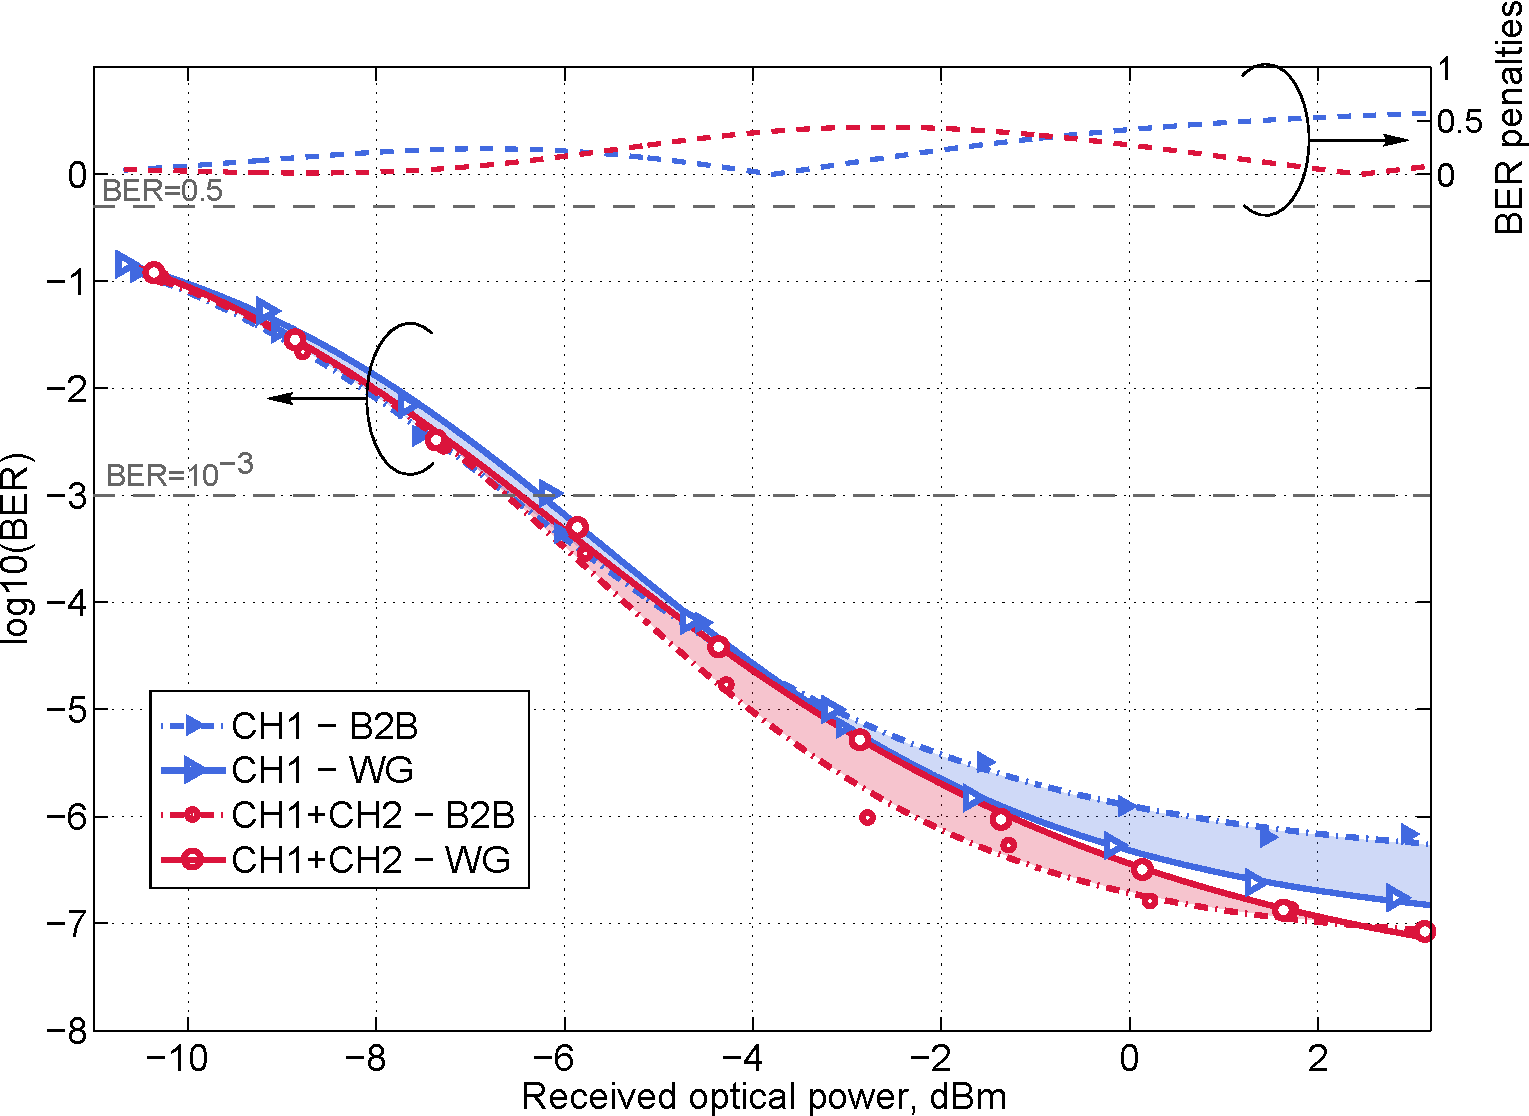
\includegraphics[height=62mm]
        {Penalties_single_or_double_channel_1549_nm.pdf}
    \end{block}
  \end{frame}

  \begin{frame}{Results and Contributinon}
               {Different wavelength regions}
    \begin{block}{1541\,–\,1556\,nm, channel spacing 0.4\,nm}
      \centering
      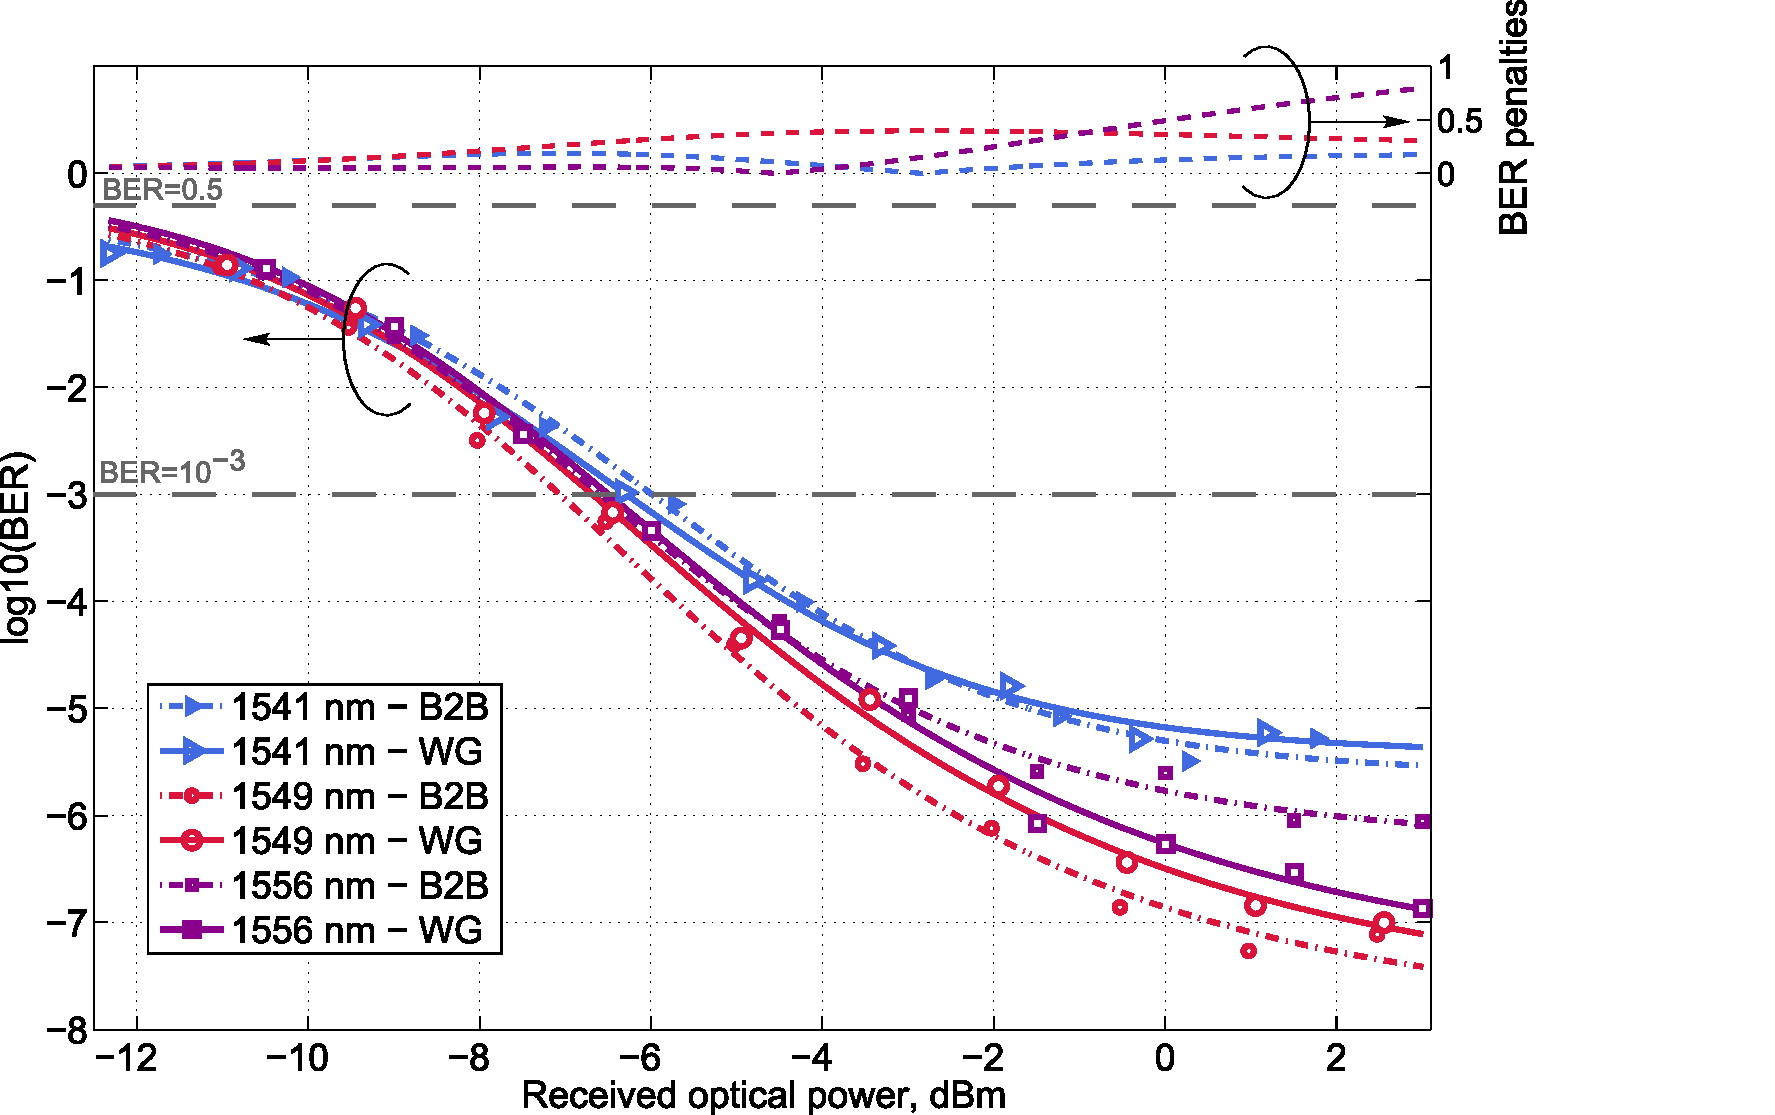
\includegraphics[height=62mm]
        {Penalties_double_channel_fixed_spacing_different_wavelength.pdf}
    \end{block}
  \end{frame}

  \begin{frame}{Results and Contributinon}
               {Different channel spacing}
    \begin{block}{1541\,nm, channel spacings 0.2\,–\,0.8\,nm}
      \centering
      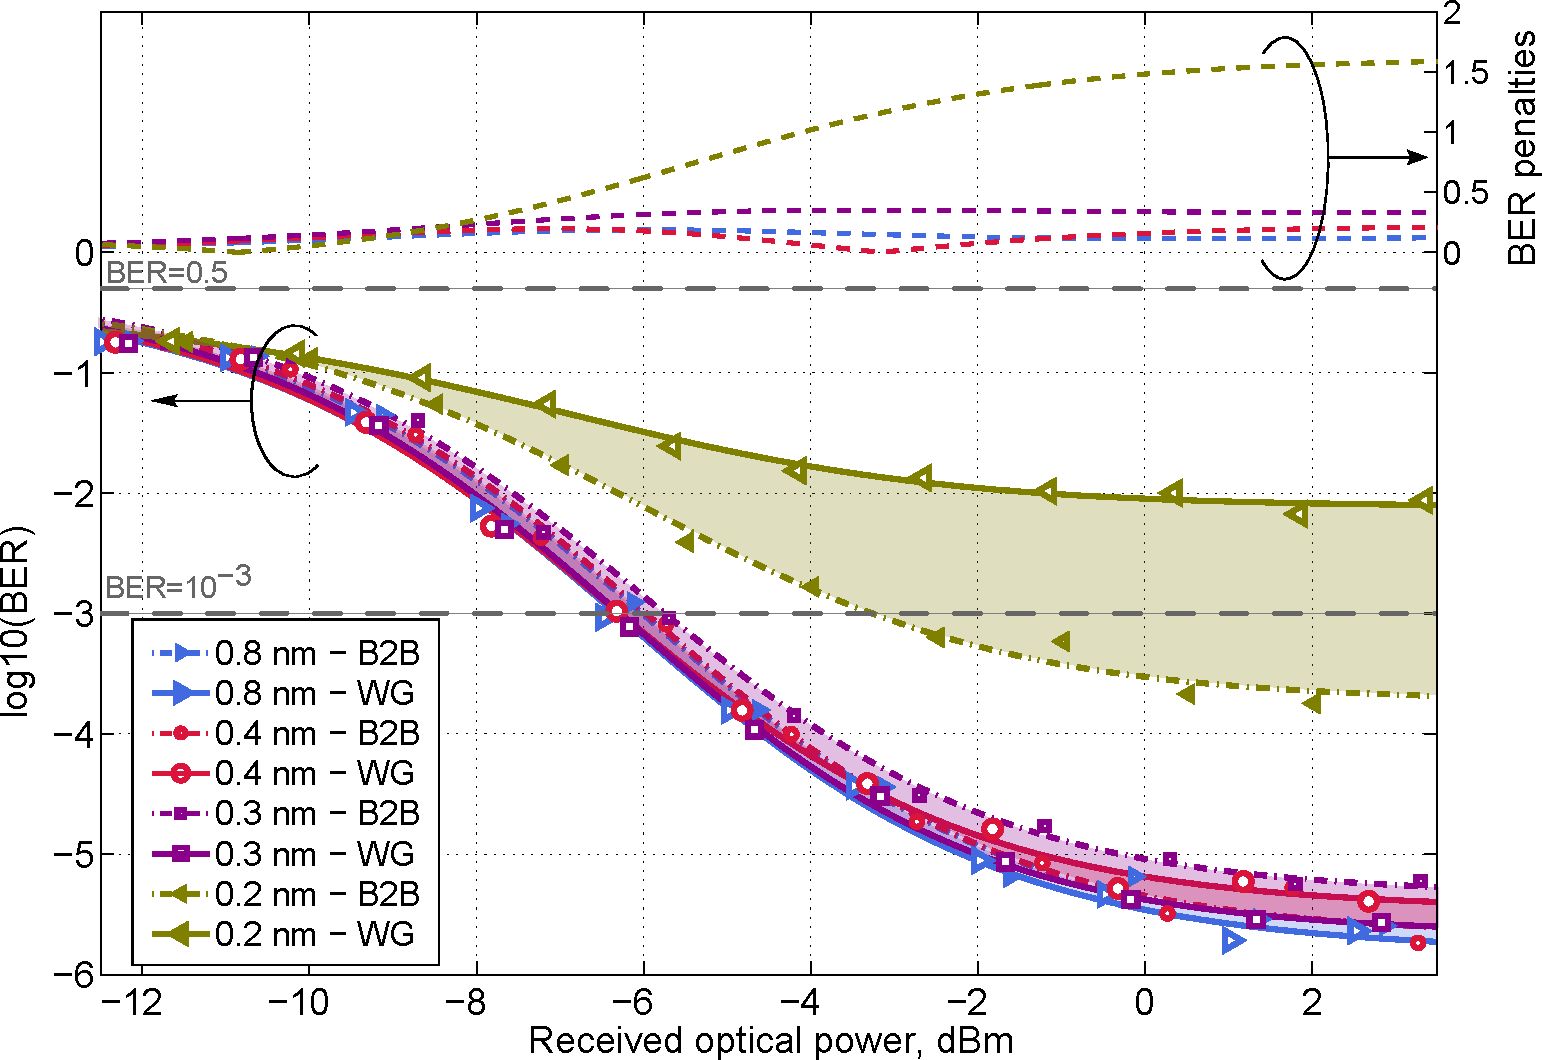
\includegraphics[height=62mm]
        {Penalties_double_channel_1541_nm_different_spacing.pdf}
    \end{block}
  \end{frame}


\section*{Summary}
%-----------------
  \begin{frame}{Summary}
    % Keep the summary *very short*.
    \begin{itemize}
    \item[\cmark] We demonstrated data transmission through the LR-DLSPPW
    \item[\cmark] BER penalties are less than 6\,dB over the 15\,nm range
    \item[\xmark] Most losses are caused by imperfect coupling
    \end{itemize}
    \begin{itemize}
    \item[\cmark] Achieved results show the applicability of LR-DLSPPW for data transmission in integrated photonics
    \end{itemize}
%    \begin{itemize}
%    \item[\ding{43}] We acknowledge nice people for their help
%    \end{itemize}
  \end{frame}



  \begin{frame}
    \begin{center}
      \begin{minipage}{0.7\textwidth}
        \begin{block}{}
          \centering
          \vspace{3mm}
          \Large \alert{Thank you for your attention!}
          \vspace{3mm}
        \end{block}
      \end{minipage}
    \end{center}
  \end{frame}

      





%##############################################################################
\appendix
\begin{frame}{Experimental setup, full diagram}
  \begin{center}
    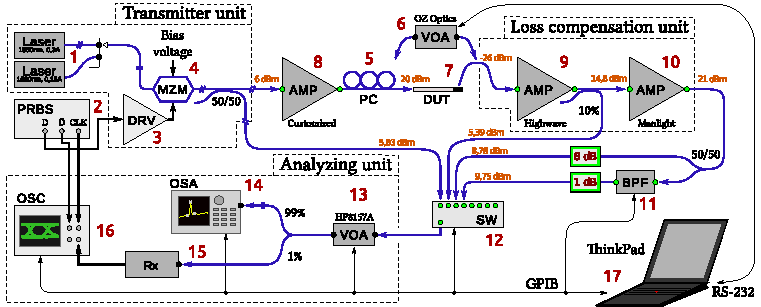
\includegraphics[width=\textwidth]{BERsetup.pdf}
  \end{center}
\end{frame}































%##############################################################################
\end{document}
%##############################################################################
%#############################################################################
% All of the following is optional and typically not needed. 
\appendix
\section<presentation>*{\appendixname}
\subsection<presentation>*{For Further Reading}

\begin{frame}[allowframebreaks]
  \frametitle<presentation>{For Further Reading}
    
  \begin{thebibliography}{10}
    
  \beamertemplatebookbibitems
  % Start with overview books.

  \bibitem{Author1990}
    A.~Author.
    \newblock {\em Handbook of Everything}.
    \newblock Some Press, 1990.
 
    
  \beamertemplatearticlebibitems
  % Followed by interesting articles. Keep the list short. 

  \bibitem{Someone2000}
    S.~Someone.
    \newblock On this and that.
    \newblock {\em Journal of This and That}, 2(1):50–100,
    2000.
  \end{thebibliography}
\end{frame}

\begin{frame}{Beamer tools – use them}
  \begin{itemize}
  \item block
  \item theorem
  \item<2> example
  \item[$\checkmark$] proof
  \item description
  \item \alert{important stuff}
  \item use columns
  \item \textbackslash{}framezoom
  \end{itemize}
\end{frame}


\begin{frame}{Enumerate, Itemize}
  There are three important points:
  \begin{enumerate}
    \item<1-> A first one,
    \item<2-> a second one with a bunch of subpoints,
  \begin{itemize}
    \item first subpoint. (Only shown from second slide on!).
    \item<3-> second subpoint added on third slide.
    \item<4-> third subpoint added on fourth slide.
  \end{itemize}
    \item<5-> and a third one.
  \end{enumerate}
\end{frame}


\begin{frame}{Structure}
  We have some text and then use \structure{\textbackslash{}structure} it it.
\end{frame}

\begin{frame}{Block}
  block of text that has a heading
  \setbeamertemplate{blocks}[default]
%  \begin{block}<⟨action specification⟩>{⟨block title⟩}<⟨action specification⟩>
  \begin{block}{block title}
  environment contents
  \end{block}
  \setbeamertemplate{blocks}[rounded][shadow=true]
  \begin{block}{block title, rounded block with shadow}
  environment contents
  \end{block}
  \begin{alertblock}{alertblock}
  environment contents
  \end{alertblock}
  \begin{exampleblock}{exampleblock}
  environment contents
  \end{exampleblock}
\end{frame}


\begin{frame}{Theorem, definition, proof}
  \begin{theorem}<1->[Theorem – Additional text]
  There exists an infinite set.
  \end{theorem}
  \begin{definition}<1->[Definition – Additional text]
  There exists an infinite set.
  \end{definition}
  \begin{proof}<2->[Proof – Additional text]
  This follows from the axiom of infinity.
  \end{proof}
  \begin{example}<3->[Natural Numbers]
  The set of natural numbers is infinite.
  \end{example}
\end{frame}




\begin{frame}{Framed and boxed text}
  Text without box
  \begin{beamercolorbox}{beamer color box}
    Text in beamercolorbox
  \end{beamercolorbox}
  
  \setbeamercolor{postit}{fg=black,bg=yellow}
  % Options can be: wd, dp, ht, left, right, center, leftskip, rightskip,
  %                 sep, colsep, colsep*, shadow, rounded, ignorebg, vmode
  \begin{beamercolorbox}[sep=1em,wd=5cm]{postit}
    Place me somewhere!
  \end{beamercolorbox}
  
  \shadowbox{shadowbox}, \doublebox{doublebox}, \ovalbox{ovalbox}, and \Ovalbox{Ovalbox}
\end{frame}


\begin{frame}{Columns}
% Column options:
  % b  will cause the bottom lines of the columns to be vertically aligned
  % c  will cause the columns to be centered vertically relative to each other.
  %       Default, unless the global option t is used.
  % onlytextwidth  is the same as totalwidth=\textwidth.
  % t  will cause the first lines of the columns to be aligned. Default if global option t is used.
  % T  is similar to the t option, but T aligns the tops of the first lines while t
  %       aligns the so-called baselines of the first lines.
  % totalwidth=⟨width⟩  will cause the columns to occupy not the whole page width,
  %       but only ⟨width⟩, all told.
  \begin{columns}[t]
    \begin{column}{5cm}
    Two\\lines.
    \end{column}
    \begin{column}{5cm}
    One line (but aligned).
    \end{column}
  \end{columns}
\end{frame}


\begin{frame}{Columns}
% \column  command
  % Starts a single column. The parameters and options are the same as for the column environment. The
  % column automatically ends with the next occurrence of \column or of a column environment or of the end
  % of the current columns environment.
  \begin{columns}
    \column[t]{5cm}
      Two\\lines.
    \column[t]{5cm}
      One line (but aligned).
  \end{columns}
\end{frame}


\begin{frame}{Abstract}
  \begin{abstract}
    This is the abstract
  \end{abstract}
\end{frame}

\begin{frame}{Columns with figure}
% \column  command
  % Starts a single column. The parameters and options are the same as for the column environment. The
  % column automatically ends with the next occurrence of \column or of a column environment or of the end
  % of the current columns environment.
  \begin{columns}
    \column[c]{0.45\textwidth}
      \begin{figure}
        
\includegraphics[width=\textwidth]{example.png}
        \caption[my caption]{An example image}
      \end{figure}
    \column[c]{0.45\textwidth}
      Look at this image. What do you see?
      \begin{itemize}
       \item Item 1
       \item Item 2
      \end{itemize}
  \end{columns}
\end{frame}


\begin{frame}{Verse and quotations}
  \begin{verse}
    This is inside of verse
  \end{verse}
  \begin{quotation}
    This is inside of quotation
  \end{quotation}
  \begin{quote}
    This is inside of quote
  \end{quote}
\end{frame}


\begin{frame}{Slide transitions}
  \begin{enumerate}
    \item<1,2> First
    \item<2> Second
    \item<3> Third
  \end{enumerate}
  \transblindshorizontal<2>
  \transblindsvertical<3>
% Other transitions are:
%\transboxin, \transboxout, \transdissolve, \transdissolve, \transglitter[direction=90], 
%\transsplitverticalin, \transsplitverticalout, \transsplithorizontalin, \transsplithorizontalin,
%\transsplithorizontalout, \transwipe, \transwipe, \transduration
\end{frame}


%##############################################################################
\end{document}
%##############################################################################